\chapter*{\textsc{Introduction}}
\addcontentsline{toc}{chapter}{\textsc{Introduction}}

	\paragraph{} L'objet de cette manipulation est de commander un système de transfert de matières premières en vrac (sable, gravier, ...) par wagonnets entre deux postes de chargement/déchargement.
	\par Les deux points essentiels illustrés par cette manipulation sont :
	
		\begin{itemize} [label=\ding{70},font=\small \color{black}]
   		\item La spécification de la commande par réseau de Petri.
   		\item Une mise en œuvre programmée de cette spécification, sur un PC en langage évolué.
  		\end{itemize}


\par Pour chaque partie de la manipulation, on modélise le système de commande par réseau de Petri et on met en œuvre cette modélisation sur PC, en utilisant le langage C et une programmation multithreads. Pour cela il faut découper le réseau de Petri en plusieurs tâches et identifier les points
de synchronisation et/ou de communication.

\par La disposition des voies empruntées par les wagonnets et la position des postes de chargement/déchargement sont données par la figure ci-dessous.

	\begin{center}
	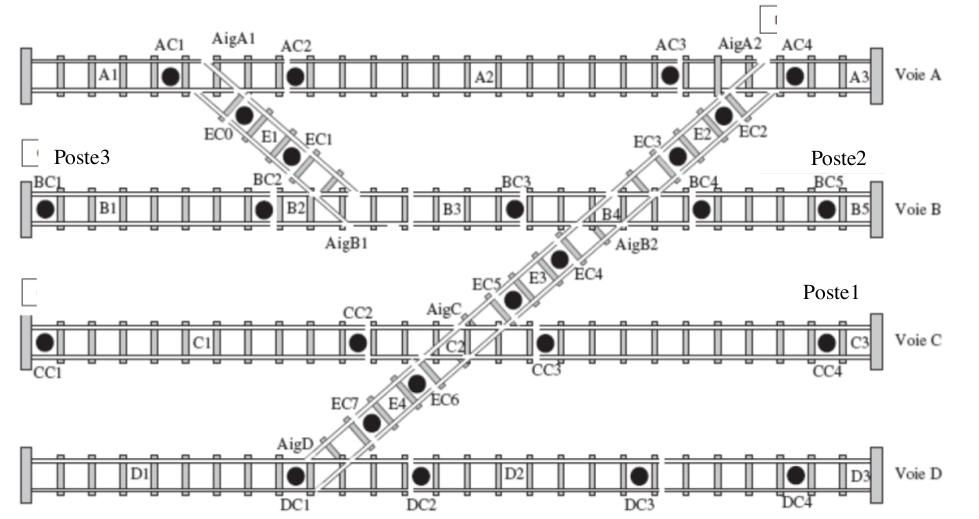
\includegraphics[scale=0.4]{maquette.png}
	\captionof{figure}{\textit{Schéma de la maquette trains. \\}}
	\label{fig4} 
	\end{center}  




